\documentclass[twoside]{book}

% Packages required by doxygen
\usepackage{fixltx2e}
\usepackage{calc}
\usepackage{doxygen}
\usepackage[export]{adjustbox} % also loads graphicx
\usepackage{graphicx}
\usepackage[utf8]{inputenc}
\usepackage{makeidx}
\usepackage{multicol}
\usepackage{multirow}
\PassOptionsToPackage{warn}{textcomp}
\usepackage{textcomp}
\usepackage[nointegrals]{wasysym}
\usepackage[table]{xcolor}

% Font selection
\usepackage[T1]{fontenc}
\usepackage[scaled=.90]{helvet}
\usepackage{courier}
\usepackage{amssymb}
\usepackage{sectsty}
\renewcommand{\familydefault}{\sfdefault}
\allsectionsfont{%
  \fontseries{bc}\selectfont%
  \color{darkgray}%
}
\renewcommand{\DoxyLabelFont}{%
  \fontseries{bc}\selectfont%
  \color{darkgray}%
}
\newcommand{\+}{\discretionary{\mbox{\scriptsize$\hookleftarrow$}}{}{}}

% Page & text layout
\usepackage{geometry}
\geometry{%
  a4paper,%
  top=2.5cm,%
  bottom=2.5cm,%
  left=2.5cm,%
  right=2.5cm%
}
\tolerance=750
\hfuzz=15pt
\hbadness=750
\setlength{\emergencystretch}{15pt}
\setlength{\parindent}{0cm}
\setlength{\parskip}{3ex plus 2ex minus 2ex}
\makeatletter
\renewcommand{\paragraph}{%
  \@startsection{paragraph}{4}{0ex}{-1.0ex}{1.0ex}{%
    \normalfont\normalsize\bfseries\SS@parafont%
  }%
}
\renewcommand{\subparagraph}{%
  \@startsection{subparagraph}{5}{0ex}{-1.0ex}{1.0ex}{%
    \normalfont\normalsize\bfseries\SS@subparafont%
  }%
}
\makeatother

% Headers & footers
\usepackage{fancyhdr}
\pagestyle{fancyplain}
\fancyhead[LE]{\fancyplain{}{\bfseries\thepage}}
\fancyhead[CE]{\fancyplain{}{}}
\fancyhead[RE]{\fancyplain{}{\bfseries\leftmark}}
\fancyhead[LO]{\fancyplain{}{\bfseries\rightmark}}
\fancyhead[CO]{\fancyplain{}{}}
\fancyhead[RO]{\fancyplain{}{\bfseries\thepage}}
\fancyfoot[LE]{\fancyplain{}{}}
\fancyfoot[CE]{\fancyplain{}{}}
\fancyfoot[RE]{\fancyplain{}{\bfseries\scriptsize Generated by Doxygen }}
\fancyfoot[LO]{\fancyplain{}{\bfseries\scriptsize Generated by Doxygen }}
\fancyfoot[CO]{\fancyplain{}{}}
\fancyfoot[RO]{\fancyplain{}{}}
\renewcommand{\footrulewidth}{0.4pt}
\renewcommand{\chaptermark}[1]{%
  \markboth{#1}{}%
}
\renewcommand{\sectionmark}[1]{%
  \markright{\thesection\ #1}%
}

% Indices & bibliography
\usepackage{natbib}
\usepackage[titles]{tocloft}
\setcounter{tocdepth}{3}
\setcounter{secnumdepth}{5}
\makeindex

% Hyperlinks (required, but should be loaded last)
\usepackage{ifpdf}
\ifpdf
  \usepackage[pdftex,pagebackref=true]{hyperref}
\else
  \usepackage[ps2pdf,pagebackref=true]{hyperref}
\fi
\hypersetup{%
  colorlinks=true,%
  linkcolor=blue,%
  citecolor=blue,%
  unicode%
}

% Custom commands
\newcommand{\clearemptydoublepage}{%
  \newpage{\pagestyle{empty}\cleardoublepage}%
}

\usepackage{caption}
\captionsetup{labelsep=space,justification=centering,font={bf},singlelinecheck=off,skip=4pt,position=top}

%===== C O N T E N T S =====

\begin{document}

% Titlepage & ToC
\hypersetup{pageanchor=false,
             bookmarksnumbered=true,
             pdfencoding=unicode
            }
\pagenumbering{alph}
\begin{titlepage}
\vspace*{7cm}
\begin{center}%
{\Large the forsaken playground }\\
\vspace*{1cm}
{\large Generated by Doxygen 1.8.13}\\
\end{center}
\end{titlepage}
\clearemptydoublepage
\pagenumbering{roman}
\tableofcontents
\clearemptydoublepage
\pagenumbering{arabic}
\hypersetup{pageanchor=true}

%--- Begin generated contents ---
\chapter{Data Structure Index}
\section{Data Structures}
Here are the data structures with brief descriptions\+:\begin{DoxyCompactList}
\item\contentsline{section}{\hyperlink{structobj}{obj} \\*Struct for obj }{\pageref{structobj}}{}
\item\contentsline{section}{\hyperlink{structObjet}{Objet} }{\pageref{structObjet}}{}
\item\contentsline{section}{\hyperlink{structvie}{vie} \\*Struct for vie }{\pageref{structvie}}{}
\end{DoxyCompactList}

\chapter{File Index}
\section{File List}
Here is a list of all documented files with brief descriptions\+:\begin{DoxyCompactList}
\item\contentsline{section}{\hyperlink{main_8c}{main.\+c} \\*Testing Program }{\pageref{main_8c}}{}
\item\contentsline{section}{\hyperlink{temps_8c}{temps.\+c} }{\pageref{temps_8c}}{}
\item\contentsline{section}{\hyperlink{temps_8h}{temps.\+h} }{\pageref{temps_8h}}{}
\end{DoxyCompactList}

\chapter{Data Structure Documentation}
\hypertarget{structobj}{}\section{obj Struct Reference}
\label{structobj}\index{obj@{obj}}


struct for obj  




{\ttfamily \#include $<$obj.\+h$>$}



\subsection{Detailed Description}
struct for obj 

The documentation for this struct was generated from the following file\+:\begin{DoxyCompactItemize}
\item 
\hyperlink{obj_8h}{obj.\+h}\end{DoxyCompactItemize}

\hypertarget{structObjet}{}\section{Objet Struct Reference}
\label{structObjet}\index{Objet@{Objet}}
\subsection*{Data Fields}
\begin{DoxyCompactItemize}
\item 
S\+D\+L\+\_\+\+Surface $\ast$ \hyperlink{structObjet_adc26449d5051fc613b8972a08a3e7bba}{image}
\item 
S\+D\+L\+\_\+\+Rect \hyperlink{structObjet_a92fd979dc6d37621933bf051914da800}{position}
\end{DoxyCompactItemize}


\subsection{Field Documentation}
\mbox{\Hypertarget{structObjet_adc26449d5051fc613b8972a08a3e7bba}\label{structObjet_adc26449d5051fc613b8972a08a3e7bba}} 
\index{Objet@{Objet}!image@{image}}
\index{image@{image}!Objet@{Objet}}
\subsubsection{\texorpdfstring{image}{image}}
{\footnotesize\ttfamily S\+D\+L\+\_\+\+Surface$\ast$ Objet\+::image}

surface. \mbox{\Hypertarget{structObjet_a92fd979dc6d37621933bf051914da800}\label{structObjet_a92fd979dc6d37621933bf051914da800}} 
\index{Objet@{Objet}!position@{position}}
\index{position@{position}!Objet@{Objet}}
\subsubsection{\texorpdfstring{position}{position}}
{\footnotesize\ttfamily S\+D\+L\+\_\+\+Rect Objet\+::position}

rectangle. 

The documentation for this struct was generated from the following file\+:\begin{DoxyCompactItemize}
\item 
\hyperlink{obj_8h}{obj.\+h}\end{DoxyCompactItemize}

\hypertarget{structvie}{}\section{vie Struct Reference}
\label{structvie}\index{vie@{vie}}


struct for vie  




{\ttfamily \#include $<$vie.\+h$>$}

\subsection*{Data Fields}
\begin{DoxyCompactItemize}
\item 
S\+D\+L\+\_\+\+Rect \hyperlink{structvie_a916050892cf1e7b8039952dcafa44825}{position}
\item 
S\+D\+L\+\_\+\+Surface $\ast$ \hyperlink{structvie_a7616ae8ecc97b7fb2d92be6a858014ad}{fond1}
\item 
S\+D\+L\+\_\+\+Surface $\ast$ \hyperlink{structvie_a6ecad7f4161cb602faa27d2de9e3ee50}{fond2}
\item 
S\+D\+L\+\_\+\+Surface $\ast$ \hyperlink{structvie_a9763ef794bb12262f5826b911d20e42b}{fond3}
\item 
S\+D\+L\+\_\+\+Surface $\ast$ \hyperlink{structvie_a0b08072b8c7ec9e1adfd6e26b4fcb39f}{fond4}
\item 
S\+D\+L\+\_\+\+Surface $\ast$ \hyperlink{structvie_adabeccdf7e33dd53ac6d85a24fc3931d}{fond5}
\item 
S\+D\+L\+\_\+\+Surface $\ast$ \hyperlink{structvie_afe9825545f1294799e27a037803d79b0}{fond6}
\end{DoxyCompactItemize}


\subsection{Detailed Description}
struct for vie 

\subsection{Field Documentation}
\mbox{\Hypertarget{structvie_a7616ae8ecc97b7fb2d92be6a858014ad}\label{structvie_a7616ae8ecc97b7fb2d92be6a858014ad}} 
\index{vie@{vie}!fond1@{fond1}}
\index{fond1@{fond1}!vie@{vie}}
\subsubsection{\texorpdfstring{fond1}{fond1}}
{\footnotesize\ttfamily S\+D\+L\+\_\+\+Surface$\ast$ vie\+::fond1}

surface. \mbox{\Hypertarget{structvie_a6ecad7f4161cb602faa27d2de9e3ee50}\label{structvie_a6ecad7f4161cb602faa27d2de9e3ee50}} 
\index{vie@{vie}!fond2@{fond2}}
\index{fond2@{fond2}!vie@{vie}}
\subsubsection{\texorpdfstring{fond2}{fond2}}
{\footnotesize\ttfamily S\+D\+L\+\_\+\+Surface$\ast$ vie\+::fond2}

surface. \mbox{\Hypertarget{structvie_a9763ef794bb12262f5826b911d20e42b}\label{structvie_a9763ef794bb12262f5826b911d20e42b}} 
\index{vie@{vie}!fond3@{fond3}}
\index{fond3@{fond3}!vie@{vie}}
\subsubsection{\texorpdfstring{fond3}{fond3}}
{\footnotesize\ttfamily S\+D\+L\+\_\+\+Surface$\ast$ vie\+::fond3}

surface. \mbox{\Hypertarget{structvie_a0b08072b8c7ec9e1adfd6e26b4fcb39f}\label{structvie_a0b08072b8c7ec9e1adfd6e26b4fcb39f}} 
\index{vie@{vie}!fond4@{fond4}}
\index{fond4@{fond4}!vie@{vie}}
\subsubsection{\texorpdfstring{fond4}{fond4}}
{\footnotesize\ttfamily S\+D\+L\+\_\+\+Surface$\ast$ vie\+::fond4}

surface. \mbox{\Hypertarget{structvie_adabeccdf7e33dd53ac6d85a24fc3931d}\label{structvie_adabeccdf7e33dd53ac6d85a24fc3931d}} 
\index{vie@{vie}!fond5@{fond5}}
\index{fond5@{fond5}!vie@{vie}}
\subsubsection{\texorpdfstring{fond5}{fond5}}
{\footnotesize\ttfamily S\+D\+L\+\_\+\+Surface$\ast$ vie\+::fond5}

surface. \mbox{\Hypertarget{structvie_afe9825545f1294799e27a037803d79b0}\label{structvie_afe9825545f1294799e27a037803d79b0}} 
\index{vie@{vie}!fond6@{fond6}}
\index{fond6@{fond6}!vie@{vie}}
\subsubsection{\texorpdfstring{fond6}{fond6}}
{\footnotesize\ttfamily S\+D\+L\+\_\+\+Surface$\ast$ vie\+::fond6}

surface. \mbox{\Hypertarget{structvie_a916050892cf1e7b8039952dcafa44825}\label{structvie_a916050892cf1e7b8039952dcafa44825}} 
\index{vie@{vie}!position@{position}}
\index{position@{position}!vie@{vie}}
\subsubsection{\texorpdfstring{position}{position}}
{\footnotesize\ttfamily S\+D\+L\+\_\+\+Rect vie\+::position}

rectangle. 

The documentation for this struct was generated from the following file\+:\begin{DoxyCompactItemize}
\item 
\hyperlink{vie_8h}{vie.\+h}\end{DoxyCompactItemize}

\chapter{File Documentation}
\hypertarget{main_8c}{}\section{main.\+c File Reference}
\label{main_8c}\index{main.\+c@{main.\+c}}


Testing Program.  


{\ttfamily \#include $<$stdio.\+h$>$}\newline
{\ttfamily \#include $<$stdlib.\+h$>$}\newline
{\ttfamily \#include $<$S\+D\+L/\+S\+D\+L.\+h$>$}\newline
{\ttfamily \#include $<$math.\+h$>$}\newline
{\ttfamily \#include $<$time.\+h$>$}\newline
{\ttfamily \#include $<$S\+D\+L/\+S\+D\+L\+\_\+image.\+h$>$}\newline
{\ttfamily \#include $<$S\+D\+L/\+S\+D\+L\+\_\+mixer.\+h$>$}\newline
{\ttfamily \#include $<$S\+D\+L/\+S\+D\+L\+\_\+ttf.\+h$>$}\newline
{\ttfamily \#include $<$string.\+h$>$}\newline
{\ttfamily \#include \char`\"{}temps.\+h\char`\"{}}\newline
Include dependency graph for main.\+c\+:
\nopagebreak
\begin{figure}[H]
\begin{center}
\leavevmode
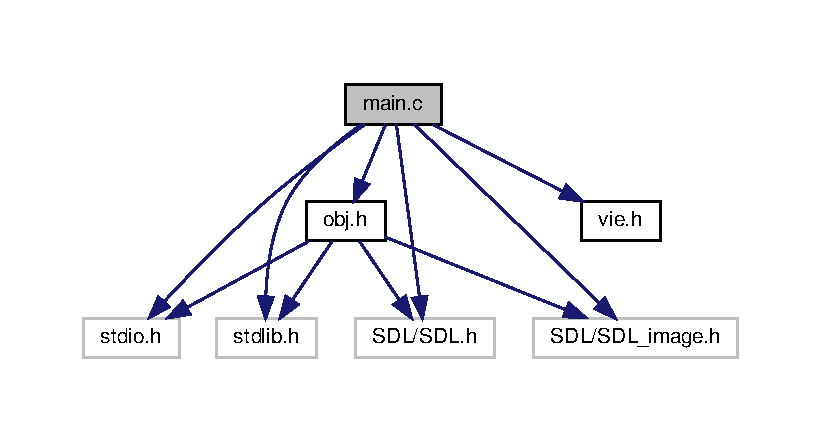
\includegraphics[width=350pt]{main_8c__incl}
\end{center}
\end{figure}
\subsection*{Functions}
\begin{DoxyCompactItemize}
\item 
\mbox{\Hypertarget{main_8c_ae66f6b31b5ad750f1fe042a706a4e3d4}\label{main_8c_ae66f6b31b5ad750f1fe042a706a4e3d4}} 
int {\bfseries main} ()
\end{DoxyCompactItemize}


\subsection{Detailed Description}
Testing Program. 

\begin{DoxyAuthor}{Author}
otail marzouk 
\end{DoxyAuthor}
\begin{DoxyVersion}{Version}
0.\+1 
\end{DoxyVersion}
\begin{DoxyDate}{Date}
mai 07, 2019
\end{DoxyDate}
Testing program for time 
\hypertarget{obj_8c}{}\section{obj.\+c File Reference}
\label{obj_8c}\index{obj.\+c@{obj.\+c}}
{\ttfamily \#include $<$stdio.\+h$>$}\newline
{\ttfamily \#include $<$stdlib.\+h$>$}\newline
{\ttfamily \#include $<$S\+D\+L/\+S\+D\+L.\+h$>$}\newline
{\ttfamily \#include $<$S\+D\+L/\+S\+D\+L\+\_\+image.\+h$>$}\newline
{\ttfamily \#include \char`\"{}obj.\+h\char`\"{}}\newline
Include dependency graph for obj.\+c\+:\nopagebreak
\begin{figure}[H]
\begin{center}
\leavevmode
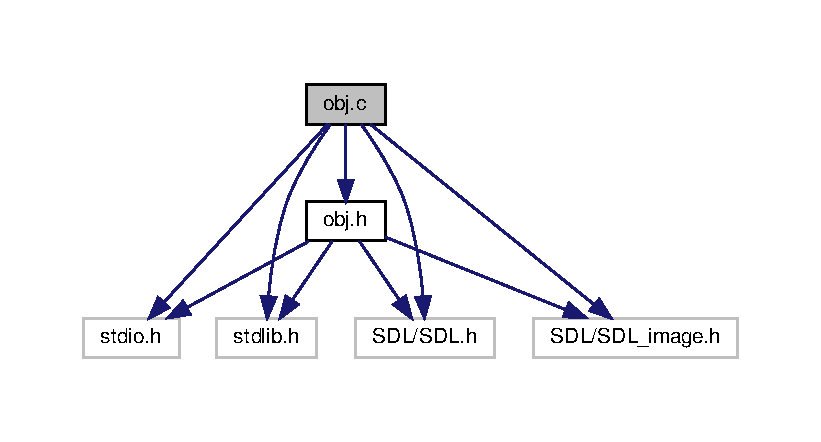
\includegraphics[width=350pt]{obj_8c__incl}
\end{center}
\end{figure}
\subsection*{Functions}
\begin{DoxyCompactItemize}
\item 
void \hyperlink{obj_8c_a33ac93d4cbcb8ad19cce6f86dde40ade}{affichage\+Obj} (\hyperlink{structObjet}{Objet} \hyperlink{structobj}{obj}, S\+D\+L\+\_\+\+Surface $\ast$screen)
\begin{DoxyCompactList}\small\item\em afficher obj . \end{DoxyCompactList}\end{DoxyCompactItemize}


\subsection{Function Documentation}
\mbox{\Hypertarget{obj_8c_a33ac93d4cbcb8ad19cce6f86dde40ade}\label{obj_8c_a33ac93d4cbcb8ad19cce6f86dde40ade}} 
\index{obj.\+c@{obj.\+c}!affichage\+Obj@{affichage\+Obj}}
\index{affichage\+Obj@{affichage\+Obj}!obj.\+c@{obj.\+c}}
\subsubsection{\texorpdfstring{affichage\+Obj()}{affichageObj()}}
{\footnotesize\ttfamily void affichage\+Obj (\begin{DoxyParamCaption}\item[{\hyperlink{structObjet}{Objet}}]{obj,  }\item[{S\+D\+L\+\_\+\+Surface $\ast$}]{screen }\end{DoxyParamCaption})}



afficher obj . 

$\ast$
\begin{DoxyParams}{Parameters}
{\em obj} & \\
\hline
{\em screen} & \\
\hline
\end{DoxyParams}
\begin{DoxyReturn}{Returns}
Nothing 
\end{DoxyReturn}

\hypertarget{obj_8h}{}\section{obj.\+h File Reference}
\label{obj_8h}\index{obj.\+h@{obj.\+h}}
{\ttfamily \#include $<$stdio.\+h$>$}\newline
{\ttfamily \#include $<$stdlib.\+h$>$}\newline
{\ttfamily \#include $<$S\+D\+L/\+S\+D\+L.\+h$>$}\newline
{\ttfamily \#include $<$S\+D\+L/\+S\+D\+L\+\_\+image.\+h$>$}\newline
Include dependency graph for obj.\+h\+:\nopagebreak
\begin{figure}[H]
\begin{center}
\leavevmode
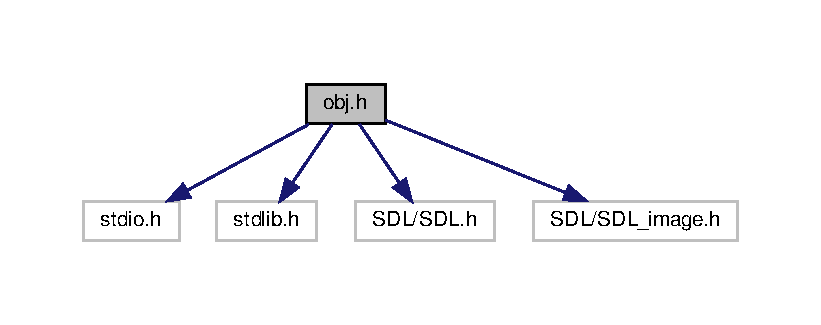
\includegraphics[width=350pt]{obj_8h__incl}
\end{center}
\end{figure}
This graph shows which files directly or indirectly include this file\+:\nopagebreak
\begin{figure}[H]
\begin{center}
\leavevmode
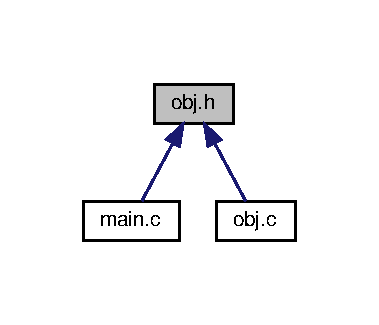
\includegraphics[width=182pt]{obj_8h__dep__incl}
\end{center}
\end{figure}
\subsection*{Data Structures}
\begin{DoxyCompactItemize}
\item 
struct \hyperlink{structObjet}{Objet}
\end{DoxyCompactItemize}
\subsection*{Functions}
\begin{DoxyCompactItemize}
\item 
void \hyperlink{obj_8h_ad8e85dcf2cfe9e95324c056906e25c19}{initialiser\+Obj} (\hyperlink{structObjet}{Objet} $\ast$\hyperlink{structobj}{obj}, char name\mbox{[}$\,$\mbox{]}, int x, int y)
\begin{DoxyCompactList}\small\item\em initialiser obj. \end{DoxyCompactList}\item 
void \hyperlink{obj_8h_a33ac93d4cbcb8ad19cce6f86dde40ade}{affichage\+Obj} (\hyperlink{structObjet}{Objet} \hyperlink{structobj}{obj}, S\+D\+L\+\_\+\+Surface $\ast$screen)
\begin{DoxyCompactList}\small\item\em afficher obj . \end{DoxyCompactList}\end{DoxyCompactItemize}


\subsection{Function Documentation}
\mbox{\Hypertarget{obj_8h_a33ac93d4cbcb8ad19cce6f86dde40ade}\label{obj_8h_a33ac93d4cbcb8ad19cce6f86dde40ade}} 
\index{obj.\+h@{obj.\+h}!affichage\+Obj@{affichage\+Obj}}
\index{affichage\+Obj@{affichage\+Obj}!obj.\+h@{obj.\+h}}
\subsubsection{\texorpdfstring{affichage\+Obj()}{affichageObj()}}
{\footnotesize\ttfamily void affichage\+Obj (\begin{DoxyParamCaption}\item[{\hyperlink{structObjet}{Objet}}]{obj,  }\item[{S\+D\+L\+\_\+\+Surface $\ast$}]{screen }\end{DoxyParamCaption})}



afficher obj . 

$\ast$
\begin{DoxyParams}{Parameters}
{\em obj} & \\
\hline
{\em screen} & \\
\hline
\end{DoxyParams}
\begin{DoxyReturn}{Returns}
Nothing 
\end{DoxyReturn}
\mbox{\Hypertarget{obj_8h_ad8e85dcf2cfe9e95324c056906e25c19}\label{obj_8h_ad8e85dcf2cfe9e95324c056906e25c19}} 
\index{obj.\+h@{obj.\+h}!initialiser\+Obj@{initialiser\+Obj}}
\index{initialiser\+Obj@{initialiser\+Obj}!obj.\+h@{obj.\+h}}
\subsubsection{\texorpdfstring{initialiser\+Obj()}{initialiserObj()}}
{\footnotesize\ttfamily void initialiser\+Obj (\begin{DoxyParamCaption}\item[{\hyperlink{structObjet}{Objet} $\ast$}]{obj,  }\item[{char}]{name\mbox{[}$\,$\mbox{]},  }\item[{int}]{x,  }\item[{int}]{y }\end{DoxyParamCaption})}



initialiser obj. 


\begin{DoxyItemize}
\item 
\begin{DoxyParams}{Parameters}
{\em name} & \\
\hline
{\em obj} & \\
\hline
{\em x} & \\
\hline
{\em y} & \\
\hline
\end{DoxyParams}
\begin{DoxyReturn}{Returns}
Nothing 
\end{DoxyReturn}

\end{DoxyItemize}
\hypertarget{vie_8c}{}\section{vie.\+c File Reference}
\label{vie_8c}\index{vie.\+c@{vie.\+c}}
{\ttfamily \#include $<$stdlib.\+h$>$}\newline
{\ttfamily \#include $<$stdio.\+h$>$}\newline
{\ttfamily \#include $<$S\+D\+L/\+S\+D\+L.\+h$>$}\newline
{\ttfamily \#include $<$S\+D\+L/\+S\+D\+L\+\_\+image.\+h$>$}\newline
{\ttfamily \#include \char`\"{}vie.\+h\char`\"{}}\newline
Include dependency graph for vie.\+c\+:\nopagebreak
\begin{figure}[H]
\begin{center}
\leavevmode
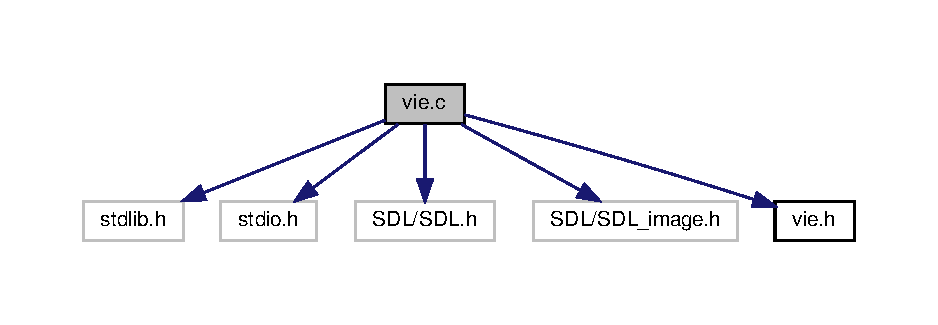
\includegraphics[width=350pt]{vie_8c__incl}
\end{center}
\end{figure}
\subsection*{Functions}
\begin{DoxyCompactItemize}
\item 
int \hyperlink{vie_8c_a7ebe6513ea3048519d01726d54a128c0}{collisionbb} (S\+D\+L\+\_\+\+Rect posj, S\+D\+L\+\_\+\+Rect posobj)
\begin{DoxyCompactList}\small\item\em collision . \end{DoxyCompactList}\item 
void \hyperlink{vie_8c_a745a3d387fc9547b8474bc07488812ef}{initialiservie} (\hyperlink{structvie}{vie} $\ast$\hyperlink{structvie}{vie})
\begin{DoxyCompactList}\small\item\em init vie. \end{DoxyCompactList}\item 
void \hyperlink{vie_8c_a4e8a988f213b277d1d87e0e595fdfd31}{affichervie} (\hyperlink{structvie}{vie} $\ast$\hyperlink{structvie}{vie}, S\+D\+L\+\_\+\+Rect $\ast$posj, S\+D\+L\+\_\+\+Rect posobj, S\+D\+L\+\_\+\+Surface $\ast$ecran, int $\ast$i)
\begin{DoxyCompactList}\small\item\em afficher vie . \end{DoxyCompactList}\end{DoxyCompactItemize}


\subsection{Function Documentation}
\mbox{\Hypertarget{vie_8c_a4e8a988f213b277d1d87e0e595fdfd31}\label{vie_8c_a4e8a988f213b277d1d87e0e595fdfd31}} 
\index{vie.\+c@{vie.\+c}!affichervie@{affichervie}}
\index{affichervie@{affichervie}!vie.\+c@{vie.\+c}}
\subsubsection{\texorpdfstring{affichervie()}{affichervie()}}
{\footnotesize\ttfamily void affichervie (\begin{DoxyParamCaption}\item[{\hyperlink{structvie}{vie} $\ast$}]{vie,  }\item[{S\+D\+L\+\_\+\+Rect $\ast$}]{posj,  }\item[{S\+D\+L\+\_\+\+Rect}]{posobj,  }\item[{S\+D\+L\+\_\+\+Surface $\ast$}]{ecran,  }\item[{int $\ast$}]{i }\end{DoxyParamCaption})}



afficher vie . 


\begin{DoxyItemize}
\item 
\begin{DoxyParams}{Parameters}
{\em vie} & \\
\hline
{\em posj} & \\
\hline
{\em posobj} & \\
\hline
{\em ecran} & \\
\hline
{\em i} & \\
\hline
\end{DoxyParams}
\begin{DoxyReturn}{Returns}
Nothing 
\end{DoxyReturn}

\end{DoxyItemize}Here is the call graph for this function\+:
\nopagebreak
\begin{figure}[H]
\begin{center}
\leavevmode
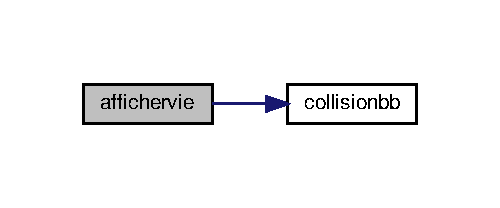
\includegraphics[width=240pt]{vie_8c_a4e8a988f213b277d1d87e0e595fdfd31_cgraph}
\end{center}
\end{figure}
\mbox{\Hypertarget{vie_8c_a7ebe6513ea3048519d01726d54a128c0}\label{vie_8c_a7ebe6513ea3048519d01726d54a128c0}} 
\index{vie.\+c@{vie.\+c}!collisionbb@{collisionbb}}
\index{collisionbb@{collisionbb}!vie.\+c@{vie.\+c}}
\subsubsection{\texorpdfstring{collisionbb()}{collisionbb()}}
{\footnotesize\ttfamily int collisionbb (\begin{DoxyParamCaption}\item[{S\+D\+L\+\_\+\+Rect}]{posj,  }\item[{S\+D\+L\+\_\+\+Rect}]{posobj }\end{DoxyParamCaption})}



collision . 

$\ast$
\begin{DoxyParams}{Parameters}
{\em posj} & \\
\hline
{\em posobj} & \\
\hline
\end{DoxyParams}
\begin{DoxyReturn}{Returns}
int 
\end{DoxyReturn}
Here is the caller graph for this function\+:
\nopagebreak
\begin{figure}[H]
\begin{center}
\leavevmode
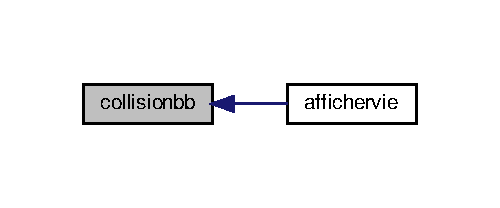
\includegraphics[width=240pt]{vie_8c_a7ebe6513ea3048519d01726d54a128c0_icgraph}
\end{center}
\end{figure}
\mbox{\Hypertarget{vie_8c_a745a3d387fc9547b8474bc07488812ef}\label{vie_8c_a745a3d387fc9547b8474bc07488812ef}} 
\index{vie.\+c@{vie.\+c}!initialiservie@{initialiservie}}
\index{initialiservie@{initialiservie}!vie.\+c@{vie.\+c}}
\subsubsection{\texorpdfstring{initialiservie()}{initialiservie()}}
{\footnotesize\ttfamily void initialiservie (\begin{DoxyParamCaption}\item[{\hyperlink{structvie}{vie} $\ast$}]{vie }\end{DoxyParamCaption})}



init vie. 

$\ast$
\begin{DoxyParams}{Parameters}
{\em vie} & \\
\hline
\end{DoxyParams}
\begin{DoxyReturn}{Returns}
Nothing 
\end{DoxyReturn}

\hypertarget{vie_8h}{}\section{vie.\+h File Reference}
\label{vie_8h}\index{vie.\+h@{vie.\+h}}
This graph shows which files directly or indirectly include this file\+:\nopagebreak
\begin{figure}[H]
\begin{center}
\leavevmode
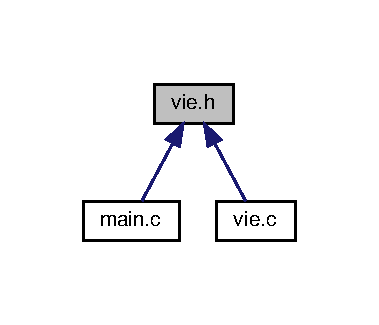
\includegraphics[width=182pt]{vie_8h__dep__incl}
\end{center}
\end{figure}
\subsection*{Data Structures}
\begin{DoxyCompactItemize}
\item 
struct \hyperlink{structvie}{vie}
\begin{DoxyCompactList}\small\item\em struct for vie \end{DoxyCompactList}\end{DoxyCompactItemize}
\subsection*{Typedefs}
\begin{DoxyCompactItemize}
\item 
\mbox{\Hypertarget{vie_8h_a5a50eadb578d4b4b9db54fdffc9b3c48}\label{vie_8h_a5a50eadb578d4b4b9db54fdffc9b3c48}} 
typedef struct \hyperlink{structvie}{vie} {\bfseries vie}
\end{DoxyCompactItemize}
\subsection*{Functions}
\begin{DoxyCompactItemize}
\item 
void \hyperlink{vie_8h_a745a3d387fc9547b8474bc07488812ef}{initialiservie} (\hyperlink{structvie}{vie} $\ast$\hyperlink{structvie}{vie})
\begin{DoxyCompactList}\small\item\em init vie. \end{DoxyCompactList}\item 
void \hyperlink{vie_8h_a4e8a988f213b277d1d87e0e595fdfd31}{affichervie} (\hyperlink{structvie}{vie} $\ast$\hyperlink{structvie}{vie}, S\+D\+L\+\_\+\+Rect $\ast$posj, S\+D\+L\+\_\+\+Rect posobj, S\+D\+L\+\_\+\+Surface $\ast$ecran, int $\ast$i)
\begin{DoxyCompactList}\small\item\em afficher vie . \end{DoxyCompactList}\item 
int \hyperlink{vie_8h_a7ebe6513ea3048519d01726d54a128c0}{collisionbb} (S\+D\+L\+\_\+\+Rect posj, S\+D\+L\+\_\+\+Rect posobj)
\begin{DoxyCompactList}\small\item\em collision . \end{DoxyCompactList}\end{DoxyCompactItemize}


\subsection{Function Documentation}
\mbox{\Hypertarget{vie_8h_a4e8a988f213b277d1d87e0e595fdfd31}\label{vie_8h_a4e8a988f213b277d1d87e0e595fdfd31}} 
\index{vie.\+h@{vie.\+h}!affichervie@{affichervie}}
\index{affichervie@{affichervie}!vie.\+h@{vie.\+h}}
\subsubsection{\texorpdfstring{affichervie()}{affichervie()}}
{\footnotesize\ttfamily void affichervie (\begin{DoxyParamCaption}\item[{\hyperlink{structvie}{vie} $\ast$}]{vie,  }\item[{S\+D\+L\+\_\+\+Rect $\ast$}]{posj,  }\item[{S\+D\+L\+\_\+\+Rect}]{posobj,  }\item[{S\+D\+L\+\_\+\+Surface $\ast$}]{ecran,  }\item[{int $\ast$}]{i }\end{DoxyParamCaption})}



afficher vie . 


\begin{DoxyItemize}
\item 
\begin{DoxyParams}{Parameters}
{\em vie} & \\
\hline
{\em posj} & \\
\hline
{\em posobj} & \\
\hline
{\em ecran} & \\
\hline
{\em i} & \\
\hline
\end{DoxyParams}
\begin{DoxyReturn}{Returns}
Nothing 
\end{DoxyReturn}

\end{DoxyItemize}Here is the call graph for this function\+:
\nopagebreak
\begin{figure}[H]
\begin{center}
\leavevmode
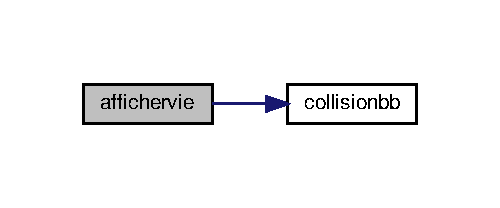
\includegraphics[width=240pt]{vie_8h_a4e8a988f213b277d1d87e0e595fdfd31_cgraph}
\end{center}
\end{figure}
\mbox{\Hypertarget{vie_8h_a7ebe6513ea3048519d01726d54a128c0}\label{vie_8h_a7ebe6513ea3048519d01726d54a128c0}} 
\index{vie.\+h@{vie.\+h}!collisionbb@{collisionbb}}
\index{collisionbb@{collisionbb}!vie.\+h@{vie.\+h}}
\subsubsection{\texorpdfstring{collisionbb()}{collisionbb()}}
{\footnotesize\ttfamily int collisionbb (\begin{DoxyParamCaption}\item[{S\+D\+L\+\_\+\+Rect}]{posj,  }\item[{S\+D\+L\+\_\+\+Rect}]{posobj }\end{DoxyParamCaption})}



collision . 

$\ast$
\begin{DoxyParams}{Parameters}
{\em posj} & \\
\hline
{\em posobj} & \\
\hline
\end{DoxyParams}
\begin{DoxyReturn}{Returns}
int 
\end{DoxyReturn}
Here is the caller graph for this function\+:
\nopagebreak
\begin{figure}[H]
\begin{center}
\leavevmode
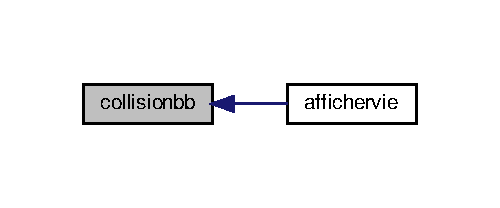
\includegraphics[width=240pt]{vie_8h_a7ebe6513ea3048519d01726d54a128c0_icgraph}
\end{center}
\end{figure}
\mbox{\Hypertarget{vie_8h_a745a3d387fc9547b8474bc07488812ef}\label{vie_8h_a745a3d387fc9547b8474bc07488812ef}} 
\index{vie.\+h@{vie.\+h}!initialiservie@{initialiservie}}
\index{initialiservie@{initialiservie}!vie.\+h@{vie.\+h}}
\subsubsection{\texorpdfstring{initialiservie()}{initialiservie()}}
{\footnotesize\ttfamily void initialiservie (\begin{DoxyParamCaption}\item[{\hyperlink{structvie}{vie} $\ast$}]{vie }\end{DoxyParamCaption})}



init vie. 

$\ast$
\begin{DoxyParams}{Parameters}
{\em vie} & \\
\hline
\end{DoxyParams}
\begin{DoxyReturn}{Returns}
Nothing 
\end{DoxyReturn}

%--- End generated contents ---

% Index
\backmatter
\newpage
\phantomsection
\clearemptydoublepage
\addcontentsline{toc}{chapter}{Index}
\printindex

\end{document}
